\section{Сокращение ресурсов при реализации моделей нелинейных искажений засчет канонического тензорного разложения}

В разделе~\ref{subsec:dynamic_dpd_2d} описана описывается метод компенсации нелинейных искажений в передатчике устройств связи в условиях динамиечского изменения режима работы УМ. Предложенный метод подразумевает компенсацию искажений путем адаптации параметров классической модели на основе двумерных полиномов Чебышева~\eqref{dpd_model_2d}. 

Основной идея данного подхода заключается в выборе признаков на входе адаптивной модели. Модель принимает на вход абсолютные значения задержанных отсчетов передатчика $|x_{n-d}|$, а также отсчеты значений входной мощности УМ $p_{n-d}$. Такой подход учитывает динамический режим работы УМ, что позволяет удовлетворить условие стационарности входного и опорного сигнала адаптивной модели и, таким образом, обеспечить сходимость алгоритма адаптации нелинейного корректора.

Результаты представленные в разделе~\ref{subsec:dynamic_dpd_2d} на рис.~\ref{fig:perform_all_data_dynamic} демонстрируют эффективность работы предложенной модели. Уровень компенсации нелинейных искажений увеличивается до 14 дБ по сравнению с классическим подходом во всем динамическом диапазоне изменения выходной мощности УМ~\eqref{powers_all_even}.

Тем не менее, многомерные модели подвержены проклятию размерности. Данный эффект подразумевает экспоненциальный рост числа параметров модели в зависимости от числа измерений~\cite{pa_models}. Действительно, число адаптивных параметров в предложенной двумерной модели~\eqref{dpd_model_2d} составляет $BP_1P_2=864$, где $B=9$ -- число веток, соответствующих различным задержкам сигнала, $P_1=8$ -- порядок измерения двумерного полинома Чебышева, соответствующего задержанному входному сигналу, $P_2=12$ -- порядок измерения двумерного полинома Чебышева $|x_{n-d}|$, соответствующего мощностному признаку $p_{n-d}$.

Таким образом, использование двумерной модели подразумевает хранение в памяти большого числа параметров, а также высокую стоимость аппаратной реализации математической модели.

В связи с этим, в данном разделе предлагается метод сокращения ресурсов аппаратной реализации на основе рангового разложения. В связи с теорией рангового разложения, описанной в разделе~\ref{subsec:tensor_canonical} однослойная двумерная нелинейная модель общего вида~\eqref{2d_nonlin_output_vector} может быть разложена в сумму из $R$ произведений одномерных моделей~\eqref{2d_nonlin_output_vector_tensor}, где $R$ -- ранг матрицы параметров адаптивной модели. 

В соответствии с векторным представлением выходных отсчетов модели на основе рангового разложения~\eqref{2d_nonlin_output_vector_tensor}, модель адаптивной компенсации~\eqref{dpd_model_2d} может быть представлена в виде:
\begin{align}
	\displaystyle &y_n=\sum_{d=-D}^{D}\sum_{r=0}^{R-1}x_{n-d}
	\begin{pmatrix}
		\displaystyle \sum_{i=0}^{P_1-1}h_{x, i, d, r}T_{i}(|x_{n-d}|)
	\end{pmatrix}
	\begin{pmatrix}
		\displaystyle \sum_{i=0}^{P_2-1}h_{p, i, d, r}T_{i}(p_{n-d})
	\end{pmatrix}, \nonumber \\
	\displaystyle &T_{i}(|x_n|)T=\cos(i\arccos(|x_n|)), \nonumber \\
	\displaystyle &T_{i}(p_n)=\cos(i\arccos(p_n)).
	\label{dpd_model_2d_tensor}
\end{align}
В выражении~\eqref{dpd_model_2d_tensor} выход двумерных функций в каждой ветке $d=\overrightarrow{-D, D}$, $z_{d, n}$ представлен в виде суммы из $R$ произведений выходных отсчетов одномерных функций $z_{x, d, n}$, $z_{p, d, n}$:
\begin{align}
	&z_{d, n}=\sum_{i=0}^{P_1-1}\sum_{j=0}^{P_2-1}h_{i, j, d}T_{i, j}(|x_{n-d}|, p_{n-d})= \nonumber \\
	=&\sum_{r=0}^{R-1}z_{x, d, n, r}z_{p, d, n, r}=\displaystyle
	\sum_{r=0}^{R-1}
	\begin{pmatrix}
		\displaystyle \sum_{i=0}^{P_1-1}h_{x, i, d, r}T_{i}(|x_{n-d}|)
	\end{pmatrix}
	\begin{pmatrix}
		\displaystyle \sum_{i=0}^{P_2-1}h_{p, i, d, r}T_{i}(p_{n-d})
	\end{pmatrix}.
	\label{dpd_model_2d_tensor_1branch}
\end{align}

Равенство~\eqref{dpd_model_2d_tensor_1branch} отражает следующее утверждение: для любого набора параметров $h_{i, j, d}$ $i=\overrightarrow{0, P_1-1}$, $j=\overrightarrow{0, P_2-1}$, $d=\overrightarrow{-D, D}$ существуют наборы параметров $h_{x, i, d, r}$ и $h_{p, j, d, r}$, $r=\overrightarrow{0, R-1}$ такие, что $z_{d, n}=z_{x, d, n, r}z_{p, d, n, r}$. То есть модель на основе раногового разложения~\eqref{dpd_model_2d_tensor} гарантированно обеспечивает уровень компенсации не меньше, чем двумерная модель~\eqref{dpd_model_2d}.

Отметим, также, что переход к модели на основе рангового разложения обеспечивает линейный рост числа параметров в зависимости от числа измерений при фиксированном ранге разложения. В текущей задаче число параметров модели:
\begin{equation}
	P_1P_2 \ (\text{2D-модель}) \rightarrow R(P_1+P_2) \ (\text{модель на основе рангового разл.}).
	\label{dimens_curse_solution}
\end{equation}
Данный подход наряду с использованием многослойных структур, является одним из методов борьбы с проклятием размерности.

Отметим, однако, что ввиду структуры~\eqref{dpd_model_2d_tensor}, критерий MSE~\eqref{mse_block} не является квадратичной функцией параметров модели на основе рангового разложения и вообще говоря не является выпуклой. По этой причине, глобальный оптимум не может быть найден за один шаг алгоритма LS~\eqref{subsec:ls}.

В то же время, в соответствиее с~\eqref{dpd_model_2d_tensor} выход модели является голоморфоной функцией~\eqref{holomorphic_error_cond}. В последующих численных экспериментах модель~\eqref{dpd_model_2d_tensor} адаптируется при помощи предложенного ранее смешанного метода Ньютона~\eqref{mixed_newton_eq_jac}, рассмотренного в разделе~\ref{subsec:mnm}.

В последующих численных экспериментах сравниваются двумерная модель~\eqref{dpd_model_2d} и модель на основе рангового разложения~\eqref{dpd_model_2d_tensor} в задаче компенсации нелинейных искажений в условиях динамического режима работы УМ. Как и в разделе~\ref{subsec:dynamic_dpd_2d} главы~\ref{chapter:methods}, описывающем решение на основе двумерной модели, данные обучающей и тестовой выборки используемые в данной задаче описаны в разделе~\ref{subsec:data_dpd_dynamic} главы~\ref{chapter:methods}.

Как и в разделе~\ref{subsec:dynamic_dpd_2d} главы~\ref{chapter:methods} порядок нелинейностей равен $P_1=8$, $P_2=8$ для измерений модуля входного сигнала $|x_n|$ и мощностных признаков УМ $p_n$ соответственно. Число параметров сравниваемых моделей собраны в таблице~\ref{tab:tensor_2d_param_num}:
\begin{table}[h]
	\centering
	\begin{tabular}{|l|c|c|c|c|}
		\hline
		Модель & Ранг $R=1$ & Ранг $R=2$ & Ранг $R=3$ & 2D \\
		\hline
		Число параметров & 180 & 360 & 540 & 864 \\
		\hline
	\end{tabular}
	\caption{Число параметров двумерной модели, а также моделей на основе рангового разложения}
	\label{tab:tensor_2d_param_num}
\end{table}

Результаты сравнения уровня компенсации нелинейных внеполосных искажений во всем динамическом диапазоне выходной мощности представлены на рис.~\ref{fig:perform_all_data_dynamic_tensor}.
\begin{figure}[!h]
	\centering
	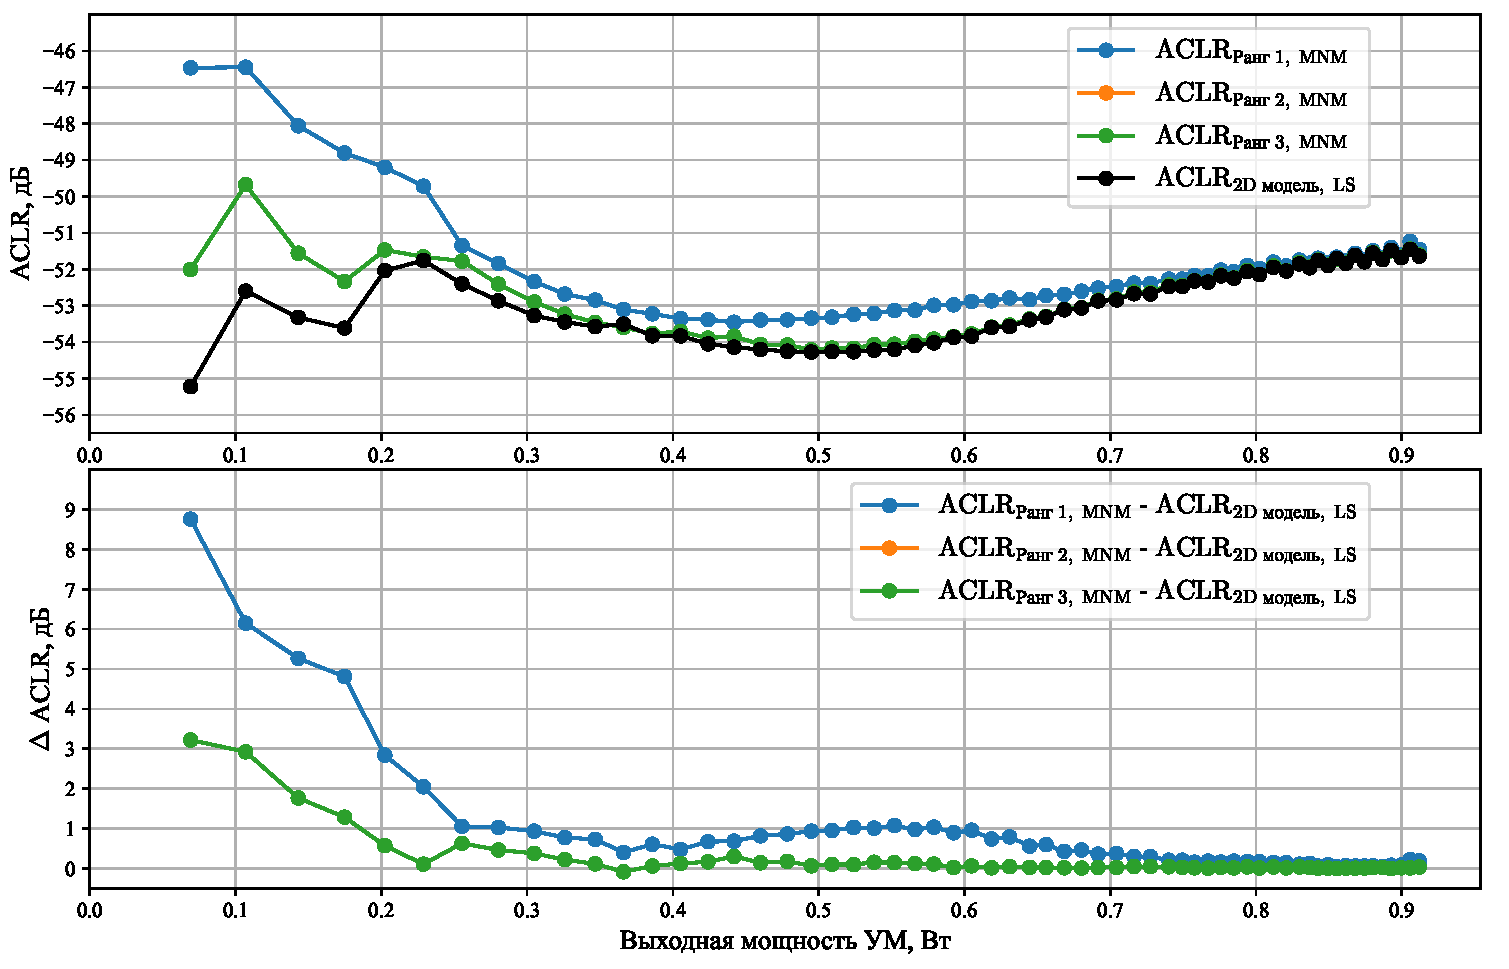
\includegraphics[width=1.0\linewidth]{figures/results/dpd_tensor/perform/perform.pdf}
	\captionsetup{justification=centering}
	\caption{Сравнение уровень компенсации внеполосных искажений в передатчике устройства связи засчет адаптации двумерной модели~\eqref{dpd_model_2d} методом LS, а также модели на основе рангового разложения~\eqref{dpd_model_2d_tensor} смешанным методом Ньютона для различных $R$}
	\label{fig:perform_all_data_dynamic_tensor}
\end{figure}

Как видно из рис.~\ref{fig:perform_all_data_dynamic_tensor} модель на основе рангового разложение матрицы параметров~\eqref{canon_tensor_decomp} двумерной модели~\eqref{2d_nonlin_output_vector_tensor} прежде всего обеспечивает компенсацию нелинейных искажений, соответствующих высоким значениям выходной мощности УМ. Результаты численных экспериментов собраны в таблице~\ref{tab:tensor_vs_2d_results}. 
\begin{table}[h!]
	\centering
	\begin{tabular}{|l|c|c|c|c|}
		\hline
		Модель & Ранг $R=1$ & Ранг $R=2$ & Ранг $R=3$ & 2D \\
		\hline
		$\max_c \Delta \text{ACLR}_c$ & 9 & 3 & -- & 0 \\
		\hline
		\makecell{$\Delta K_R$ (\%)} & 79.2 & 58.3 & 37.5 & 0 \\
		\hline
	\end{tabular}
	\caption{Сравнение характеристик моделей}
	\label{tab:tensor_vs_2d_results}
\end{table}

Из таблицы~\ref{tab:tensor_vs_2d_results} видно, что максимальное ухудшение компенсации в соседнем канале $\Delta\text{ACLR}\approx9$ dB по сравнению с двумерной моделью соответствует выходной мощности 70 мВт при использовании рангового разложения с $R=1$. Максимальное ухудшение компенсации в соседнем канале $\Delta\text{ACLR}\approx3$ dB соответствует выходной мощности 70 мВт при использовании рангового разложения с $R=2$. При $R=3$, $\Delta\text{ACLR}\approx$ dB для выходной мощности УМ мВт. 

Кроме того, в таблице~\ref{tab:tensor_vs_2d_results} посчитан процент уменьшения числа параметров по сравнению в двумерной моделью (таблица~\ref{tab:tensor_2d_param_num}) по формуле:
\begin{equation}
	\Delta K_R=\frac{K_{2D}-K_{R-rank}}{K_{2D}}\cdot100\%.
	\label{tensor_param_num_reduction}
\end{equation}
Предложенная модель позволяет уменьшить число параметров на 79.2\%, 58.3\%, 37.5\% для $R=1$, $R=2$, $R=3$ соответственно по сравнению с 2D-моделью.

Таким образом, модель на основе рангового разложения позволяет существенно уменьшить ресурсы необходимые для аппаратной реализации до 80\% засчет ухудшения предсказательной способности до 9 дБ для малой выходной мощности УМ. При достаточном ранге $R=3$ разложения уменьшение ресурсов меньше и составляет 37.5\%, при этом ухудшение предсказательной способности составляет менее дБ.